
%(BEGIN_QUESTION)
% Copyright 2009, Tony R. Kuphaldt, released under the Creative Commons Attribution License (v 1.0)
% This means you may do almost anything with this work of mine, so long as you give me proper credit

Read and outline the ``Derivative and Integral Control Actions'' subsection of the ``Analog Electronic PID Controllers'' section of the ``Closed-Loop Control'' chapter in your {\it Lessons In Industrial Instrumentation} textbook.  Note the page numbers where important illustrations, photographs, equations, tables, and other relevant details are found.  Prepare to thoughtfully discuss with your instructor and classmates the concepts and examples explored in this reading.

\underbar{file i04310}
%(END_QUESTION)





%(BEGIN_ANSWER)


%(END_ANSWER)





%(BEGIN_NOTES)

Capacitors naturally differentiate voltage, yielding a current whose magnitude is proportional to the rate-of-change of voltage over time:

$$I = C {dV \over dt}$$

If we place capacitors in the negative feedback network of an operational amplifier, we can get that opamp circuit to either differentiate or integrate.  If the input signal must pass through a capacitor first, the opamp will {\it differentiate}.  If the feedback signal from the opamp's output must pass through a capacitor, the opamp will {\it integrate}.

\vskip 10pt

\noindent
{\bf Differentiator formula:}

$$V_{out} = -RC {dV_{in} \over dt} \hskip 50pt V_{out} = -\tau_d {dV_{in} \over dt}$$

\vskip 10pt

\noindent
{\bf Integrator formula:}

$$\Delta V_{out} = -{1 \over RC} \int V_{in} \> dt \hskip 50pt \Delta V_{out} = -{1 \over \tau_i} \int V_{in} \> dt$$

$$V_{out} = -{1 \over RC} \int V_{in} \> dt + V_0 \hskip 50pt V_{out} = -{1 \over \tau_i} \int V_{in} \> dt + V_0$$








\vskip 20pt \vbox{\hrule \hbox{\strut \vrule{} {\bf Suggestions for Socratic discussion} \vrule} \hrule}

\begin{itemize}
\item{} Reasoning from the formula $I = C {dV \over dt}$, plot sine waves for AC voltage and current as they relate to a capacitor, and use these plots to explain why current leads voltage for a capacitor.
\item{} How to modify a differentiator circuit to yield more aggressive action?
\item{} How to modify an integrator circuit to yield more aggressive action?
\item{} Explore the general principle of negative feedback systems, whereby the transfer function of the feedback loop is inverted at the amplifier output.  A voltage-{\it divided} feedback, by this principle, yields a voltage {\it gain} at the opamp output.
\begin{itemize}

\item{} What happens if we feed back the opamp's voltage signal {\it times 3} to its inverting input? 
\item{} What happens if we feed back the {\it square root} of the opamp's voltage signal to its inverting input?
\item{} What happens if we feed back the {\it logarithm} of the opamp's voltage signal to its inverting input?
\end{itemize}
\end{itemize}

\vfil \eject

$$\includegraphics[width=15.5cm]{i04310x01.eps}$$
















\vfil \eject

\noindent
{\bf Prep Quiz:}

The heart of integral and derivative (I and D) actions in an analog electronic controller is the {\it capacitor}, which relates voltage and current by the following equation:

\begin{itemize}
\item{} $V = IR$
\vskip 10pt
\item{} ${dI \over dt} = CV$
\vskip 10pt
\item{} $I = C{dV \over dt}$
\vskip 10pt
\item{} $Q = CV$
\vskip 10pt
\item{} $X = {1 \over 2\pi fC}$
\vskip 10pt
\item{} $P = IV$
\end{itemize}


%INDEX% Reading assignment: Lessons In Industrial Instrumentation, closed-loop control (D and I analog electronic control)

%(END_NOTES)


